%\subsection{Approximate Euler-Maruyama scheme}\label{subsec:euler_maruyama}

\subsection{The sample-based approximate scheme}\label{sec:sample_based}

In the gradient descent \eqref{eq:discretized_noisy_flow}, the vector field depends on the target distribution $\mu$ and the current distribution $\nu_n$ at each iteration $n$, to which we do not have access. This suggests a simple approximate scheme, based on samples of the two latter distributions, that can be computed in practice. 
Given i.i.d. samples $(X^i_0)_{1\leq i\leq N}$ and $(Y^{m})_{1\leq m\leq M}$ from $\nu_0$ and $\mu$ and step-size $\gamma$, the approximate scheme iteratively updates the particles $i$ using the following update equation: 
\begin{align}\label{eq:euler_maruyama}
X_{n+1}^{i} = X_n^i -\gamma \nabla f_{\hat{\mu},\hat{\nu}_n}(X_n^i+\beta_n U_n^i)
\end{align}
where $U_{n}^{i}$ are i.i.d standard gaussians and $\hat{\mu}$, $\hat{\nu}_n$ denote respectively the empirical distributions of $(Y^{m})_{1\leq m\leq M}$ and $(X^i_n)_{1\leq i\leq N}$. One nice property about this scheme is that $\nabla f_{\hat{\mu},\hat{\nu}_n}(.)$ can be evaluated easily by:
\begin{equation}
%\nabla f_{\hat{\mu},\hat{\nu}_n}(X_n^i+\beta_n U_n^i) = \frac{1}{M}\sum\limits_{m=1}^M \nabla_2 k(Y_m,X_n^i+\beta_n U_n^i)-\frac{1}{N}\sum\limits_{j=1}^N \nabla_2 k(X_n^j+\beta_n U_n^j,X_n^i+\beta_n U_n^i)
\nabla f_{\hat{\mu},\hat{\nu}_n}(.) = \frac{1}{M}\sum\limits_{m=1}^M \nabla_2 k(Y_m,.)-\frac{1}{N}\sum\limits_{j=1}^N \nabla_2 k(X_n^j,.)
\end{equation}
where $\nabla_2k(x,.)$ denotes the gradient of $k$ w.r.t. the second variable for any $x \in \X$.
However, unlike the algorithms derived from the Negative Sobolev distance or the Sliced Wasserstein gradient flows (see respectively \cite{Mroueh:2019,Simsekli:2018}), \cref{eq:euler_maruyama} is computationally less expensive. Indeed the cost of each iteration is $O((M+N)N)$ and uses $O(M+N)$ in memory.
\cref{eq:euler_maruyama} can be seen as a particle version of \cref{eq:euler_scheme} and one would expect it to converge towards the its population version as $M$ and $N$ goes to infinity. This is made more formal in the following theorem.
%\begin{theorem}\label{prop:convergence_euler_maruyama}
%Under the same conditions as in \cref{prop:convergence_euler_scheme} and for any $\frac{T}{\gamma}\geq n\geq 0$:
%\begin{equation}
%\mathbb[E][W_2(\hat{\nu}_n,\nu_n)] = \frac{1}{2}(\frac{var(\mu)^\frac{1}{2}}{M} + \frac{(var(\nu_0)^\frac{1}{2})}{N}e^{LT})(e^LT-1)
%\end{equation}
%Where $M(\gamma k)$ is a constant that only depends on $\gamma n$ and the choice of the kernel $k$.
%\end{theorem}
\begin{theorem}\label{prop:convergence_euler_maruyama}
	For any $\frac{T}{\gamma}\geq n\geq 0$:\aknote{check conditions}
\[
\mathbb{E}[W_{2}(\hat{\nu}_{n},\nu_{n})]\leq \frac{1}{2}\left(\frac{1}{\sqrt{N}}(B+var(\nu_{0})^{\frac{1}{2}})e^{LT}+\frac{1}{\sqrt{M}}var(\mu))\right)(e^{LT}-1)
\]
\end{theorem}
Notice that since we do not have access to true samples of $\nu_n$ at each iteration $n$, we have adopted the common approach (sometimes referred to as \textit{mean-field interaction} in mathematical physics and stochastic analysis) which considers the system of  $N$ interacting particles $(X_n^{1,N}, X_n^{2,N}, \dots, X_n^{N,N})$ and their empirical distribution in order to approximate $\nu_n$.
\cref{prop:convergence_euler_maruyama} tries to control the propagation of the chaos at each iteration and uses techniques from \cite{Jourdain:2007}, however, the proof is much simpler since it is provided in discrete time. Notice also that these rates remain true when no noise is added to the updates, i.e. for the original flow when $B=0$. A proof is provided in \cref{prop:propagation_chaos}. The dependence in $\sqrt{N}$ underlines the fact that our algorithm could be interesting as a sampling algorithm when one only has access to samples of $\mu$ (see \cref{subsec:kl_flow}).

%\begin{remark}
%Two settings are usually encountered in the sampling literature: \textit{density-based}, i.e. the target $\mu$ is known up to a constant, or \textit{sample-based}, i.e. we only have access to a set of samples $X \sim \mu$. The Unadjusted Langevin Algorithm (ULA), which involves a time-discretized version of the Langevin diffusion (see \cref{remark:gradient_flow}), seems much more suitable for first setting, since it only requires the knowledge of $\nabla \log \mu$, whereas our algorithm requires the knowledge of $\mu$ (since $\nabla f_{\mu, \nu_n}$ involves an integration over $\mu$). However, in the sample-based setting, it may be difficult to adapt the ULA algorithm, since it would require firstly to estimate $\nabla \log(\mu)$ based on a set of samples of $\mu$, before plugging this estimate in the update of the algorithm. This problem, sometimes referred to as \textit{score estimation} in the literature, has been the subject of a lot of work but remains hard especially in high dimensions (see \cite{sutherland2017efficient},\cite{li2018gradient},\cite{shi2018spectral}). In contrast, the discretized flow of the $MMD^2$ presented in this section seems naturally adapted to the sample-based setting.
%\end{remark}












%
%
%
%\cref{eq:mcKean_Vlasov_process} suggests a time discretized approximation to \cref{eq:continuity_mmd} which will be analyzed in \cref{sec:convergence_mmd_flow}:
%\begin{align}\cref{eq:time_discretized_flow}
%	X_{n+1} = X_n - \gamma \nabla f_{\nu_n}(X_n) \qquad X_0\sim \nu_0
%\end{align}
%where $\gamma >0$ is the step-size. Using standard techniques from
% 
%
%\paragraph{Modified gradient flow}
%
%
\textbf{Experiments}


\begin{figure}[ht]
	\centering
	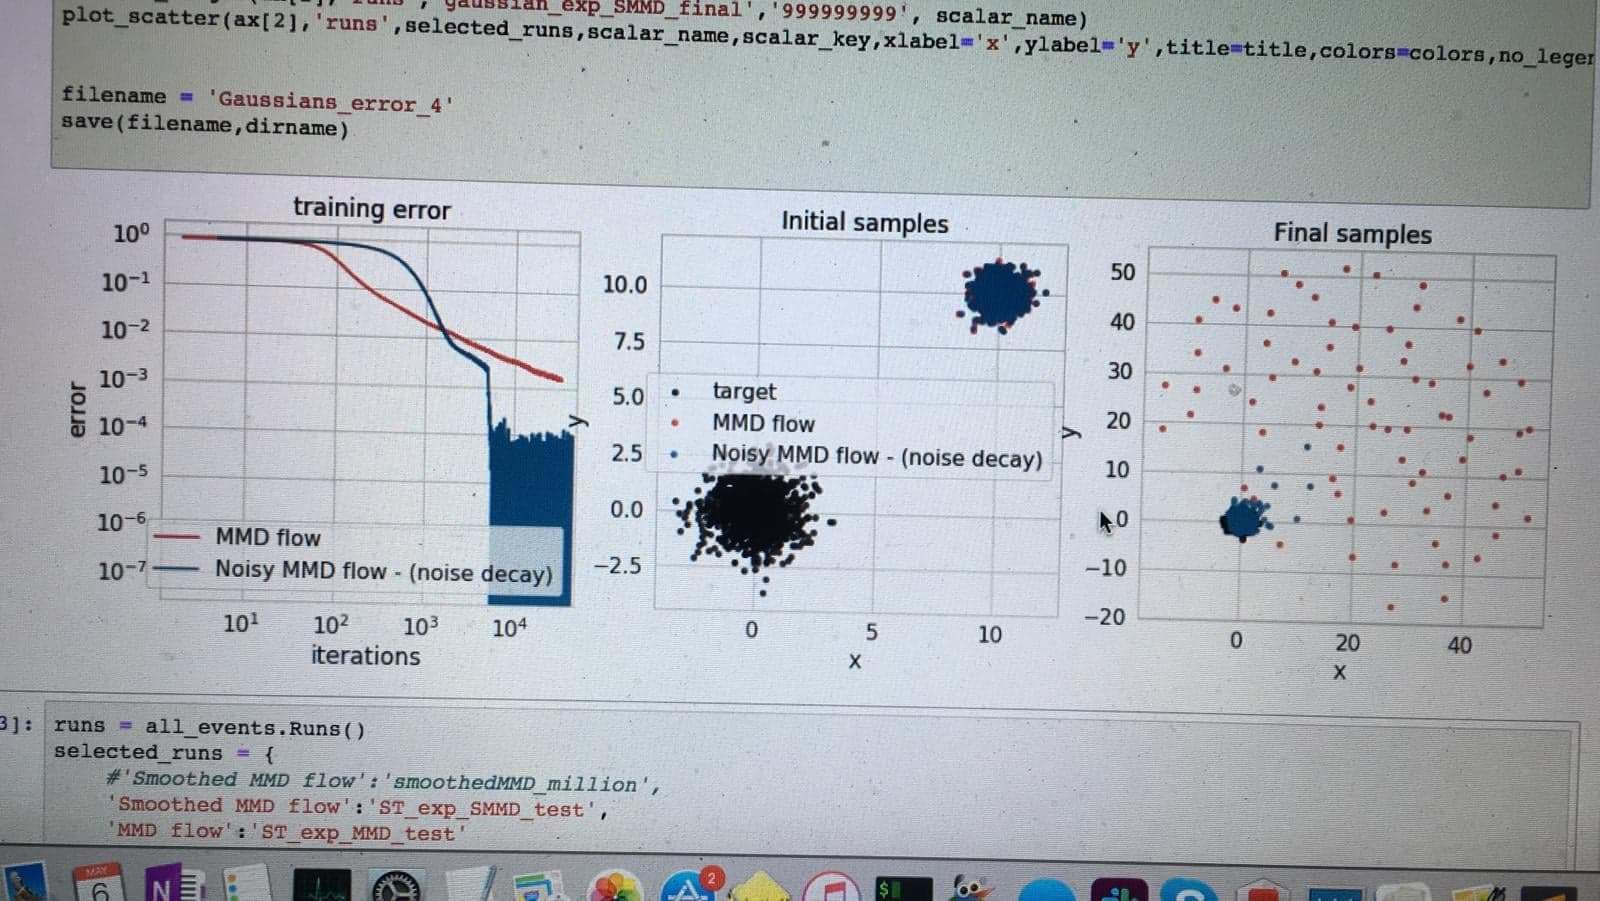
\includegraphics[width=0.5\linewidth]{experiments.jpg}
	\caption{An illustration of the performance of the regular versus noisy MMD flow.}
	\label{fig:experiments}
\end{figure}

Figure \ref{fig:experiments} shows the result of the experiment.









